\documentclass[../../../main.tex]{subfiles}
\begin{document}

%%%%%%%%%%%%%%%%%%%%%%%%%%%%%%%%%%%%%%%%%
%%%%%%%%%%%%%%%%%%%%%%%%%%%%%%%%%%%%%%%%%
%%%%%%%%%%%%%%%%%%%%%%%%%%%%%%%%%%%%%%%%%
\chapter{Confidence intervals}

In many situations, we don't know the mean of the population, and it would be too expensive or just too infeasible to actually compute the true mean of the population. So, we must take a sample, and compute the mean of that. 

The main question we are concerned with is this: how representative is this sample of the larger population? Well, what does it mean to be ``representative''? We can be pretty exact here. What we mean is this: how close is the sample mean to the population mean? 

It turns out that we can actually compute that, within a certain range (plus or minus some amount), our sample mean is close to the population mean, and we can even be 95\% confident of this (or 68\% confident, or some other percentage of confidence).

When we say that we are XX\% confident that our sample mean (plus or minus some amount) captures the population mean, we call this a \vocab{confidence interval}.


%%%%%%%%%%%%%%%%%%%%%%%%%%%%%%%%%%%%%%%%%
%%%%%%%%%%%%%%%%%%%%%%%%%%%%%%%%%%%%%%%%%
\section{The concept of the interval}

Imagine that we have a population and we don't know the mean of the population. For example, we want to know the mean height of all high school students in Delaware, and we don't know this value. 

Calculating it would be too costly, so we need to take a sample. Suppose, then, that we randomly select 30 students, and measure their heights. Then we compute the mean of those 30 heights, which turns out to be (say) 66 inches. So we have the sample mean.

What are the chances that our sample mean is the same as the population mean? What are the chances that the mean height we calculated for our 30 students is exactly the same as the mean height of all high school students in Delaware? 

It seems impossible. Perhaps (if we're very lucky), we'd get very close. But there's just no way we'd get the exact same mean from our sample. 

But, what if we take the sample mean, plus or minus some extra amount, to account for the error in our sample? For example, suppose we take our sample mean, and then add/subtract 5, so that we have the range or interval from 61 to 71 inches? 

Now, what are the chances that this interval contains the population mean? Now the chances seem much better, right? It seems much more likely that our sample mean (plus or minus 5), captures the population mean. 

This is the idea of an interval. We want to know how close our sample mean is to the population mean, but since a sample will always have some error in it, the exact sample mean is unlikely to match the population mean. So we widen the range a bit, to account for the error. This range is what we mean when we talk about an interval.


%%%%%%%%%%%%%%%%%%%%%%%%%%%%%%%%%%%%%%%%%
%%%%%%%%%%%%%%%%%%%%%%%%%%%%%%%%%%%%%%%%%
\section{The concept of confidence}

How wide do we make our interval, and how sure can we be that it will include the population mean? Amazingly, we can be quite precise. The reason has to do with the fact that sampling distributions are normal, and we know a lot about normal curves.

Here is a normal curve, with some standard deviations marked on it:


\begin{center}
  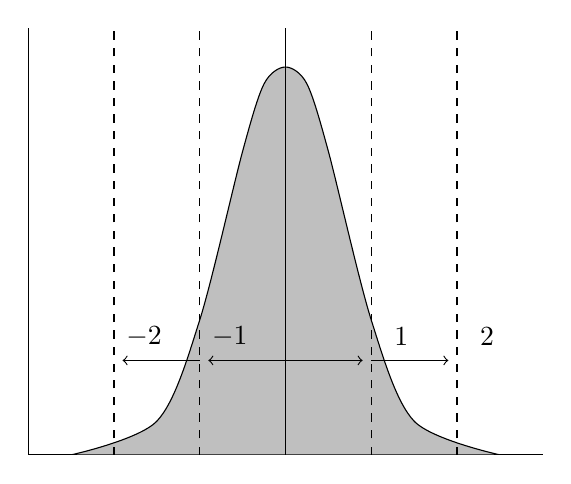
\begin{tikzpicture}
    \begin{axis}[
      axis lines*=left,
      ytick=\empty,
      xtick=\empty,
      height=7cm,
      enlarge y limits={value=0.1,upper},
      ]
      \addplot[smooth, fill=lightgray, domain=0:10] 
        coordinates{
          (0, 0) (2, 0.5) (3, 2) (4, 4.5) (4.5, 5.5)
          (5, 5.75)
          (5.5, 5.5) (6, 4.5) (7, 2) (8, 0.5) (10, 0)} 
        \closedcycle;
        
      \draw (5, 0) -- (5, 10);
      \node at (5.5, 1.75) {$\populationmean$};
      
      \draw[dashed] (7, 0) -- (7, 10);
      \node at (7.7, 1.75) {$1\populationstdev$};
      \draw[->] (5, 1.4) -- (6.8, 1.4);
      \draw[dashed] (9, 0) -- (9, 10);
      \node at (9.7, 1.75) {$2\populationstdev$};
      \draw[->] (7, 1.4) -- (8.8, 1.4);
      
      \draw[dashed] (3, 0) -- (3, 10);
      \node at (3.7, 1.75) {$-1\populationstdev$};
      \draw[->] (5, 1.4) -- (3.2, 1.4);
      \draw[dashed] (1, 0) -- (1, 10);
      \node at (1.7, 1.75) {$-2\populationstdev$};
      \draw[->] (3, 1.4) -- (1.2, 1.4);
    \end{axis}
  \end{tikzpicture}
\end{center}

\noindent
Think about what we know:

\begin{itemize}

  \item We know that 68\% of the values of a normal curve are contained within 1 STDEV from the mean.

  \item We know that the mean of a sampling distribution is the same as the mean of the population.

  \item We also know that the sampling distribution of sample means is made up of all the sample means taken from the larger population.

  \item So, no matter which mean we get from our sample, we know that there is a 68\% chance that it is one of those sample means that falls within 1 STDEV of the population mean.

\end{itemize}

\noindent
Of course, we don't know where the real mean is, so we don't know how close our sample mean actually is to the real population mean. Perhaps our sample is the one that falls in the following spot on the distribution (where we've marked a red line):

\begin{center}
  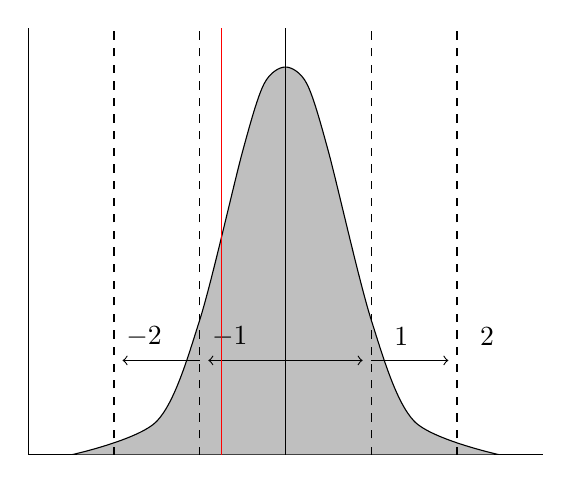
\begin{tikzpicture}
    \begin{axis}[
      axis lines*=left,
      ytick=\empty,
      xtick=\empty,
      height=7cm,
      enlarge y limits={value=0.1,upper},
      ]
      \addplot[smooth, fill=lightgray, domain=0:10] 
        coordinates{
          (0, 0) (2, 0.5) (3, 2) (4, 4.5) (4.5, 5.5)
          (5, 5.75)
          (5.5, 5.5) (6, 4.5) (7, 2) (8, 0.5) (10, 0)} 
        \closedcycle;
        
      \draw (5, 0) -- (5, 10);
      \node at (5.5, 1.75) {$\populationmean$};
      
      \draw[dashed] (7, 0) -- (7, 10);
      \node at (7.7, 1.75) {$1\populationstdev$};
      \draw[->] (5, 1.4) -- (6.8, 1.4);
      \draw[dashed] (9, 0) -- (9, 10);
      \node at (9.7, 1.75) {$2\populationstdev$};
      \draw[->] (7, 1.4) -- (8.8, 1.4);
      
      \draw[dashed] (3, 0) -- (3, 10);
      \node at (3.7, 1.75) {$-1\populationstdev$};
      \draw[->] (5, 1.4) -- (3.2, 1.4);
      \draw[dashed] (1, 0) -- (1, 10);
      \node at (1.7, 1.75) {$-2\populationstdev$};
      \draw[->] (3, 1.4) -- (1.2, 1.4);
      
      \draw[color=red] (3.5, 0) -- (3.5, 10);
    \end{axis}
  \end{tikzpicture}
\end{center}

If that's our sample mean, well then it's within 1 STDEV of the mean. But of course, we don't know if it's fallen in this spot or not, because we don't know the actual mean. Our sample mean might very well be a different one, for example here: 

\begin{center}
  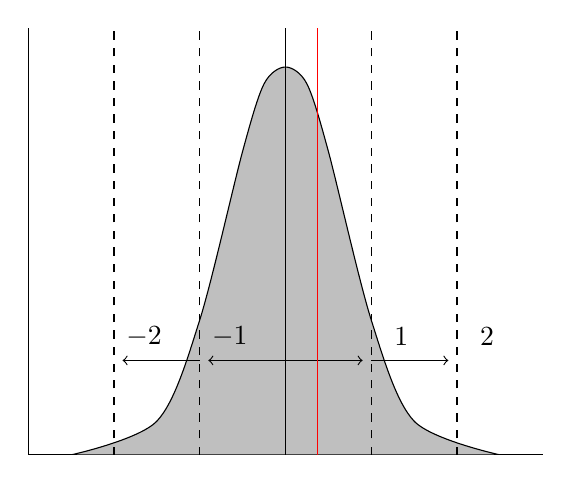
\begin{tikzpicture}
    \begin{axis}[
      axis lines*=left,
      ytick=\empty,
      xtick=\empty,
      height=7cm,
      enlarge y limits={value=0.1,upper},
      ]
      \addplot[smooth, fill=lightgray, domain=0:10] 
        coordinates{
          (0, 0) (2, 0.5) (3, 2) (4, 4.5) (4.5, 5.5)
          (5, 5.75)
          (5.5, 5.5) (6, 4.5) (7, 2) (8, 0.5) (10, 0)} 
        \closedcycle;
        
      \draw (5, 0) -- (5, 10);
      \node at (5.5, 1.75) {$\populationmean$};
      
      \draw[dashed] (7, 0) -- (7, 10);
      \node at (7.7, 1.75) {$1\populationstdev$};
      \draw[->] (5, 1.4) -- (6.8, 1.4);
      \draw[dashed] (9, 0) -- (9, 10);
      \node at (9.7, 1.75) {$2\populationstdev$};
      \draw[->] (7, 1.4) -- (8.8, 1.4);
      
      \draw[dashed] (3, 0) -- (3, 10);
      \node at (3.7, 1.75) {$-1\populationstdev$};
      \draw[->] (5, 1.4) -- (3.2, 1.4);
      \draw[dashed] (1, 0) -- (1, 10);
      \node at (1.7, 1.75) {$-2\populationstdev$};
      \draw[->] (3, 1.4) -- (1.2, 1.4);
      
      \draw[color=red] (5.75, 0) -- (5.75, 10);
    \end{axis}
  \end{tikzpicture}
\end{center}

If it were that sample mean, then it would also be within 1 STDEV of the mean. But again, we don't know that it falls here. It might very well fall in a different place. For example, here:

\begin{center}
  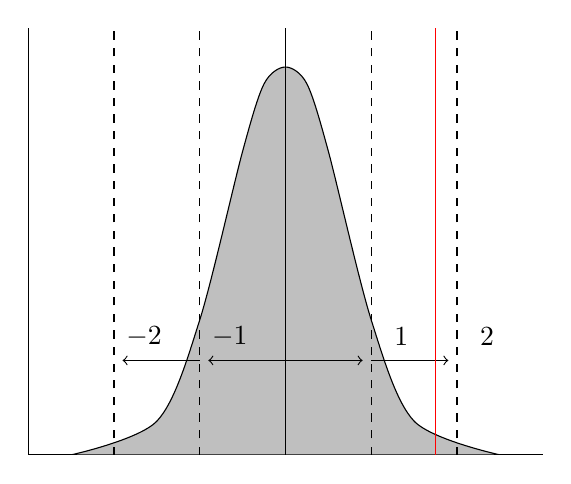
\begin{tikzpicture}
    \begin{axis}[
      axis lines*=left,
      ytick=\empty,
      xtick=\empty,
      height=7cm,
      enlarge y limits={value=0.1,upper},
      ]
      \addplot[smooth, fill=lightgray, domain=0:10] 
        coordinates{
          (0, 0) (2, 0.5) (3, 2) (4, 4.5) (4.5, 5.5)
          (5, 5.75)
          (5.5, 5.5) (6, 4.5) (7, 2) (8, 0.5) (10, 0)} 
        \closedcycle;
        
      \draw (5, 0) -- (5, 10);
      \node at (5.5, 1.75) {$\populationmean$};
      
      \draw[dashed] (7, 0) -- (7, 10);
      \node at (7.7, 1.75) {$1\populationstdev$};
      \draw[->] (5, 1.4) -- (6.8, 1.4);
      \draw[dashed] (9, 0) -- (9, 10);
      \node at (9.7, 1.75) {$2\populationstdev$};
      \draw[->] (7, 1.4) -- (8.8, 1.4);
      
      \draw[dashed] (3, 0) -- (3, 10);
      \node at (3.7, 1.75) {$-1\populationstdev$};
      \draw[->] (5, 1.4) -- (3.2, 1.4);
      \draw[dashed] (1, 0) -- (1, 10);
      \node at (1.7, 1.75) {$-2\populationstdev$};
      \draw[->] (3, 1.4) -- (1.2, 1.4);
      
      \draw[color=red] (8.5, 0) -- (8.5, 10);
    \end{axis}
  \end{tikzpicture}
\end{center}

If it fell there, it would not be within 1 STDEV of the mean. If this were our sample, we would be quite a long way off from the population mean. 

We can't know for sure which sample our sample mean is. But, because the sampling distribution has a normal curve, we can be sure that 68\% of the values contained in that curve fall within 1 STDEV of the mean. So we can be sure that there is a 68% chance that our sample mean is within 1 STDEV of the population mean. 

Notice that we don't know if we are, or are not within 1 STDEV of the population mean. Perhaps our sample mean does fall within that 68\% of the curve's values, or perhaps our sample mean is one of the 32\% of the values that fall outside that middle 68\%. We don't know, and probably never will. 

All we can be sure about here is that we have a 68\% \emph{chance} that we are within the 1 STDEV range. In other words, we can be sure of the \emph{probability} of our sample mean's proximity to the real mean.

This percentage chance is what we call our \vocab{confidence level}. Here we've pointed out that we can have a confidence level of 68\% that our sample mean falls within 1 STDEV of the population mean. 


%%%%%%%%%%%%%%%%%%%%%%%%%%%%%%%%%%%%%%%%%
%%%%%%%%%%%%%%%%%%%%%%%%%%%%%%%%%%%%%%%%%
\section{Constructing a confidence interval}

Constructing a confidence interval is straightforward. First, you take your sample, and compute the mean from that sample. So, we compute a sample mean.

Then, we decide what level of confidence we want. For now, let's suppose we want a confidence level of 68\%. We know that this lines up with plus or minus 1 STDEV from the mean. So, we take our sample mean, and we add/subtract 1 STDEV to it, to get an interval. Let's call the bottom number A, and the top number B.

Once we have all that, we can then say that we are 68\% confident that the unknown population mean is within the interval from A to B.

To do this, we need to be able to calculate how much 1 STDEV is, for the particular sampling distribution we are working with. For any sampling distribution, the STDEV (which we call the standard error) is defined by:

\begin{equation*}
  \StdErr/ = \frac{\populationstdev}{\sqrt{\samplesize/}}
\end{equation*}

\noindent
To calculate this, we need to know the sample size $\samplesize/$, and the population STDEV $\populationstdev$. But, assuming we know both of those, then we can compute the standard deviaton ($\StdErr/$) for the sampling distribution, and then we can add/subtract one of those from our sample mean.


%%%%%%%%%%%%%%%%%%%%%%%%%%%%%%%%%%%%%%%%%
%%%%%%%%%%%%%%%%%%%%%%%%%%%%%%%%%%%%%%%%%
\section{An example}

Consider the following:

\begin{itemize}

  \item Suppose we don't know the mean height of all high school students in the state of Delaware, but suppose we know the standard deviation for the population. It is 5 (so $\populationstdev = 5$). 

  \item Suppose now that we want to estimate the true mean height of the entire population. To do this, we take a sample of 30 high school students (so the sample size is 30, i.e., $\samplesize/ = 30$). 

  \item Suppose we measure the heights of all 30 students, and we find that the mean of our 30 students comes out to be 66.3 inches. So $\samplemean/ = 66.3$. 

\end{itemize}

\noindent
Suppose now that we want to come up with a condidence interval that estimates the true population mean with 68\% confidence. How do we do this? We follow these steps:

\begin{enumerate}

  \item we must compute how big a standard deviation is for this sampling distribution. The formula for that is: 

  \begin{equation*}
    \StdErr/ = \frac{\populationstdev}{\sqrt{\samplesize/}}
  \end{equation*}

  \noindent
  If we plug in our sample size (30) and the population STDEV (5), we can compute the STDEV (also called the standard error) for the sampling distribution:

  \begin{equation*}
    \StdErr/ = \frac{\populationstdev}{\sqrt{\samplesize/}} = \frac{5}{\sqrt{30}} = 0.91
  \end{equation*}

  \noindent
  So, the standard deviation (also called the standard error) for a sampling distribution of 30 specimens is 0.91. 

  \item Next, we add one $\StdErr/$ to our sample mean, to get the top number of the interval: 

  \begin{equation*}
    \samplemean{x} + (1 * \StdErr/) = 66.3 + 0.91 = 67.21
  \end{equation*}

  \noindent
  And we subtract one $\StdErr/$ from our sample mean, to get the bottom number of the interval:

  \begin{equation*}
    \samplemean{x} - (1 * \StdErr/) = 66.3 - 0.91 = 65.39
  \end{equation*}  

  \item Now that we have the top and bottom numbers of the interval, we can state our confidence interval:

  \begin{quote}
    The \textbf{68\% confidence interval} for this population is $\mathbf{66.3 \pm 0.91}$, \\
    i.e., \textbf{(65.39, 67.21)}. \\

    In words: We estimate with 68\% confidence that the true mean height for all high school students in Delaware is between 65.39 and 67.21 inches.
  \end{quote}

\end{enumerate}


%%%%%%%%%%%%%%%%%%%%%%%%%%%%%%%%%%%%%%%%%
%%%%%%%%%%%%%%%%%%%%%%%%%%%%%%%%%%%%%%%%%
\section{$\alpha$ and $Z_{\frac{\alpha}{2}}$}

In a normal curve, the area outside the confidence interval we care about is called $\alpha$ (that's the lowercase Greek letter alpha). If we are interested in a 68\% confidence interval, then $\alpha$ will be the 32\% in the tails outside of that. Of course, half of 32\% will be on each side (hence $\frac{\alpha}{2} = 16\%$ on each side). Here is a picture:

    [Picture]

\noindent
The boundary lines that separate the two colors are sometimes called the \vocab{error bounds}, or the \vocab{error bound means} (or EDMs for short). To refer to the number of z-scores from the mean up to the EDMs, we can write $Z_{\frac{alpha}{2}}$, and we substitute in the actual area of $\frac{\alpha}{2}$. 

Some examples:

\begin{itemize}
  \item If we are interested in a 68\% confidence interval, then $\alpha = .32$, and $\frac{\alpha}{2} = 0.16$, so $Z_{0.16}$.
  \item If we are interested in a 95\% confidence interval, then $\alpha = .05$, and $\frac{\alpha}{2} = 0.025$, so $Z_{0.025}$.
\end{itemize}


%%%%%%%%%%%%%%%%%%%%%%%%%%%%%%%%%%%%%%%%%
%%%%%%%%%%%%%%%%%%%%%%%%%%%%%%%%%%%%%%%%%
\section{The formula}

We can summarize the above calculations with the following formula:

\begin{equation*}
  \samplemean{x} + \text{z-score}(\StdErr/) < \populationmean < \samplemean{x} + \text{z-score}(\StdErr/)
\end{equation*}

\noindent
This says that the population mean (i.e., $\populationmean$) is between the sample mean $\samplemean{x}$ plus and minus the number of STDEVs we care about (where the number of STDEVs is the z-score multiplied by the $\StdErr/$).

Since the $\StdErr/$ for the sampling distribution is defined as $\frac{\populationstdev}{\sqrt{\samplesize/}}$, and since the z-score we care about can be written as $Z_{\frac{\alpha}{2}}$, we can substitute those in to get this:

\begin{equation*}
  \samplemean{x} - Z_{\frac{\alpha}{2}}(\frac{\populationstdev}{\sqrt{\samplesize/}}) < \populationmean < \samplemean{x} + Z_{\frac{\alpha}{2}}(\frac{\populationstdev}{\sqrt{\samplesize/}})
\end{equation*}

\noindent
That is the way that it is often written in textbooks and other references.


%%%%%%%%%%%%%%%%%%%%%%%%%%%%%%%%%%%%%%%%%
%%%%%%%%%%%%%%%%%%%%%%%%%%%%%%%%%%%%%%%%%
\section{The 95\% confidence interval}

Instead of a 68\% confidence level, we might want a 95\% confidence level. Well, that's 1.96 STDEVs (although sometimes people fudge this and just call it 2 STDEVs).

To construct a confidence interval for the same sample, but one with a 95\% confidence interval, we have to add/subtract 1.96 STDEVs from the mean. Since 1 STDEV is 0.91, 1.96 will be almost twice that much:

\begin{equation*}
  0.91 * 1.96 = 1.78  
\end{equation*}

\noindent
And then the top and bottom numbers of the interval will be these:

\begin{align*}
  66.3 + 1.78 = 68.08 \\
  66.3 - 1.78 = 64.52
\end{align*}

\noindent
So, we can state our 95\% confidence interval like this:

\begin{quote}
  The \textbf{95\% confidence interval} for this population is $\mathbf{66.3 \pm 1.78}$, \\
  i.e., \textbf{(64.52, 68.08)}. \\

  In words: We estimate with 95\% confidence that the true mean height for all high school students in Delaware is between 64.52 and 68.08 inches.
\end{quote}


%%%%%%%%%%%%%%%%%%%%%%%%%%%%%%%%%%%%%%%%%
%%%%%%%%%%%%%%%%%%%%%%%%%%%%%%%%%%%%%%%%%
\section{Common z-scores}

Here are some common z-scores that correspond to common confidence intervals:

\begin{itemize}
  \item 68\% = 1
  \item 90\% = 1.645
  \item 95\% = 1.96
  \item 99\% = 2.56
\end{itemize}

\noindent
So, if you want a confidence interval of 68\%, you multiply the computed $\StdErr/$ for your sampling distribution by $\pm 1$. If you want a confidence interval of 90\%, you multiply the computed $\StdErr/$ by $\pm 1.645$. Likewise for 95\% and 99\%.


%%%%%%%%%%%%%%%%%%%%%%%%%%%%%%%%%%%%%%%%%
%%%%%%%%%%%%%%%%%%%%%%%%%%%%%%%%%%%%%%%%%
\section{Using the sample's STDEV}

Sometimes we do not know the STDEV of the entire population (that is, we do not $\populationstdev$). If your sample size is large enough (rough guide: if it has at least 30 specimens), then we can simply compute the standard deviation of the \emph{sample} (which we abbreviate as $\samplestdev$), and then substitute that into the above formulas in place of $\populationstdev$. 

So, for large samples (30 or bigger), we can simply use $\samplestdev$ instead of $\populationstdev$.


\end{document}
